\chapter{Análise Estatística }\label{ape:intervencoes}

\textbf{Questão 1: Os itens recomendados corresponderam com os meus interesses.}

\begin{figure}[htb]
  \caption{\label{fig:questao1-boxplot}Boxplot da questão 1}
  \begin{center}
      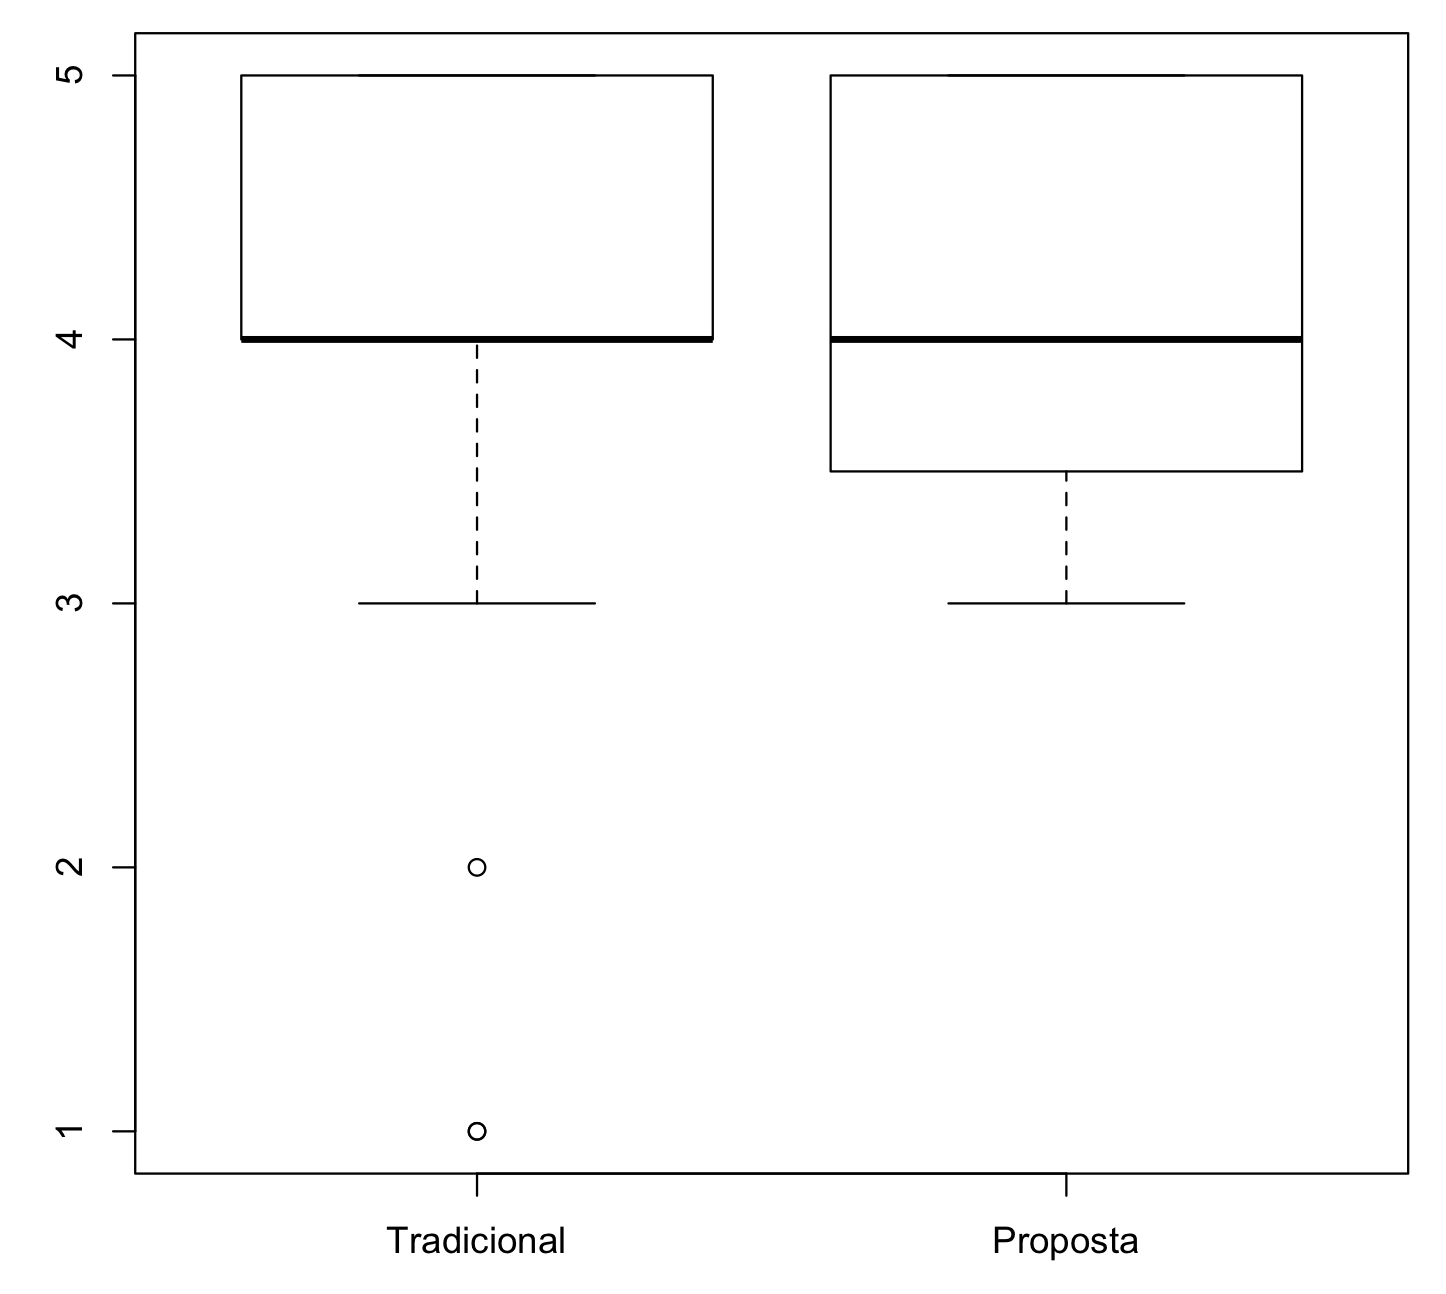
\includegraphics[scale=0.6]{./Figuras/questao1-boxplot.png}
  \end{center}
  \legend{Fonte: O autor.}
\end{figure}

Wilcoxon rank sum test with continuity correction

data:  $data\_61\_tradicional$ and $data\_61\_proposta$\\
W = 404, p-value = 0.5635\\
alternative hypothesis: true location shift is not equal to 0


\newpage\newpage
\textbf{Questão 2: Os itens recomendados para mim são diversificados (o sistema se preocupa em trazer itens diferentes a cada recomendação).}

\begin{figure}[htb]
  \caption{\label{fig:questao2-boxplot}Boxplot da questão 2}
  \begin{center}
      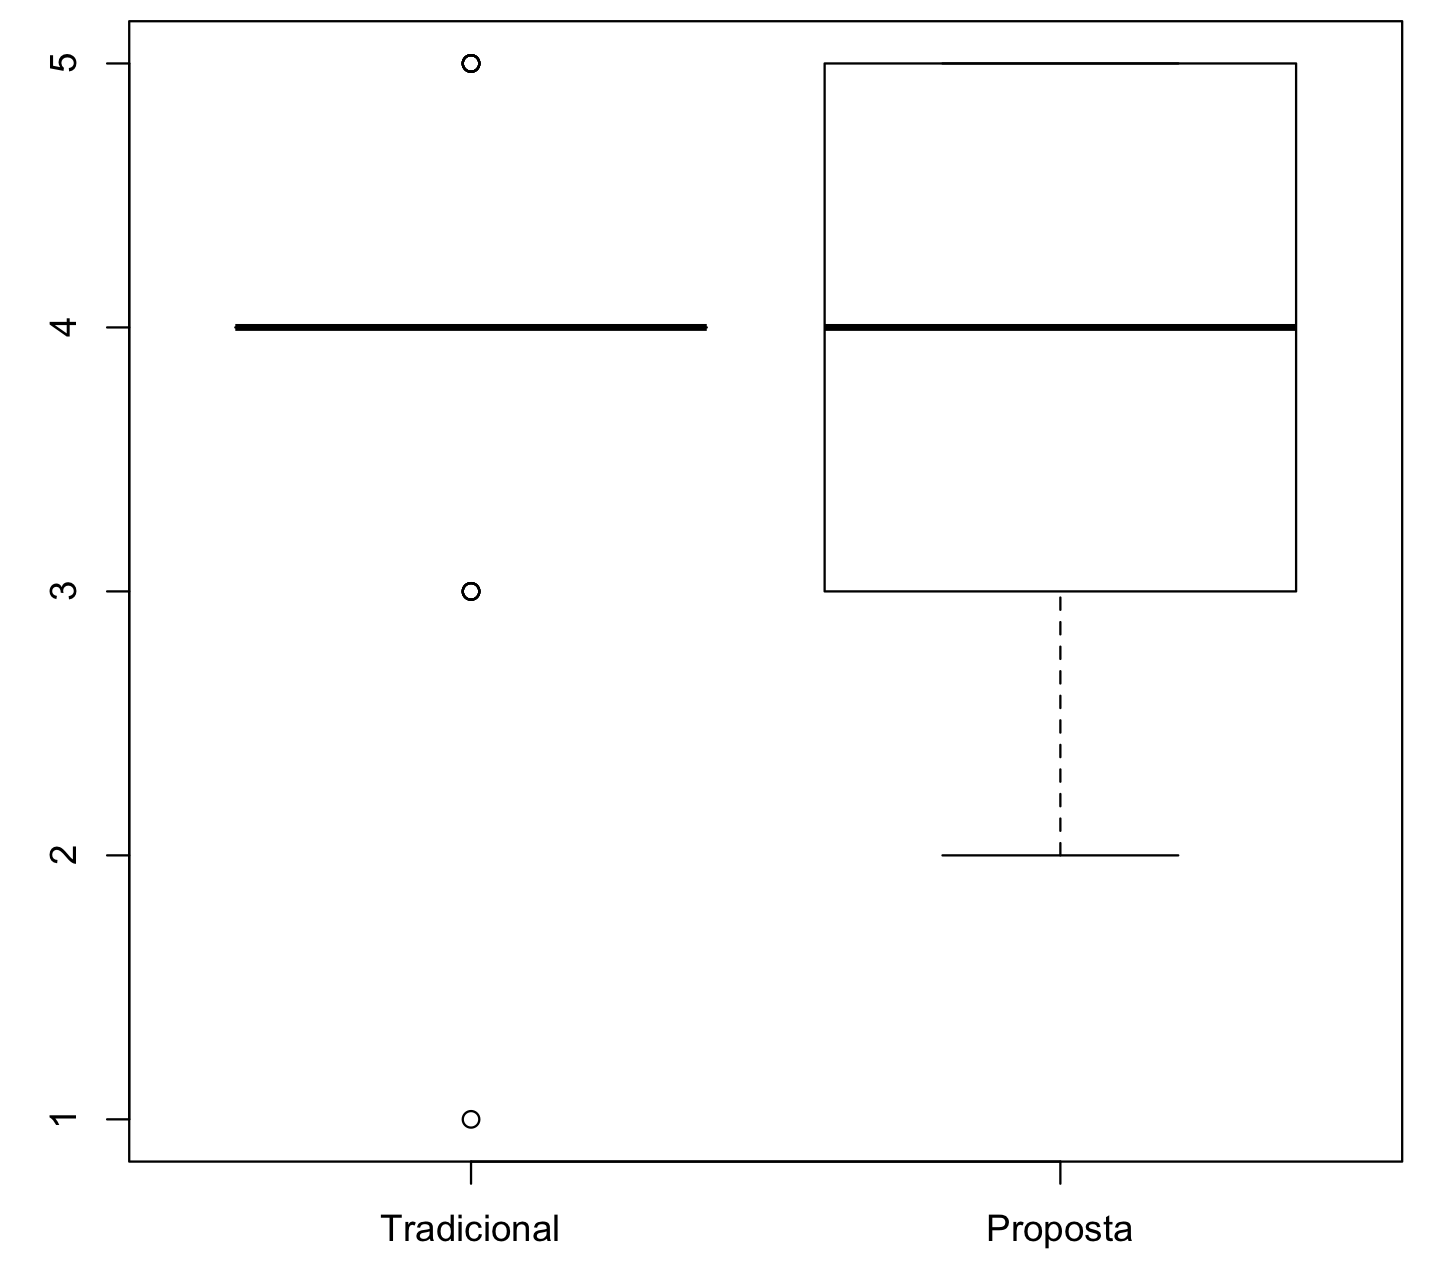
\includegraphics[scale=0.6]{./Figuras/questao2-boxplot.png}
  \end{center}
  \legend{Fonte: O autor.}
\end{figure}

Wilcoxon rank sum test with continuity correction

data:  $data\_62\_tradicional$ and $data\_62\_proposta$\\
W = 376.5, p-value = 0.8178\\
alternative hypothesis: true location shift is not equal to 0

\newpage
\textbf{Questão 3: Os itens recomendados corresponderam aos  interesses e necessidades que eu tinha no momento.}

\begin{figure}[htb]
  \caption{\label{fig:questao3-boxplot}Boxplot da questão 3}
  \begin{center}
      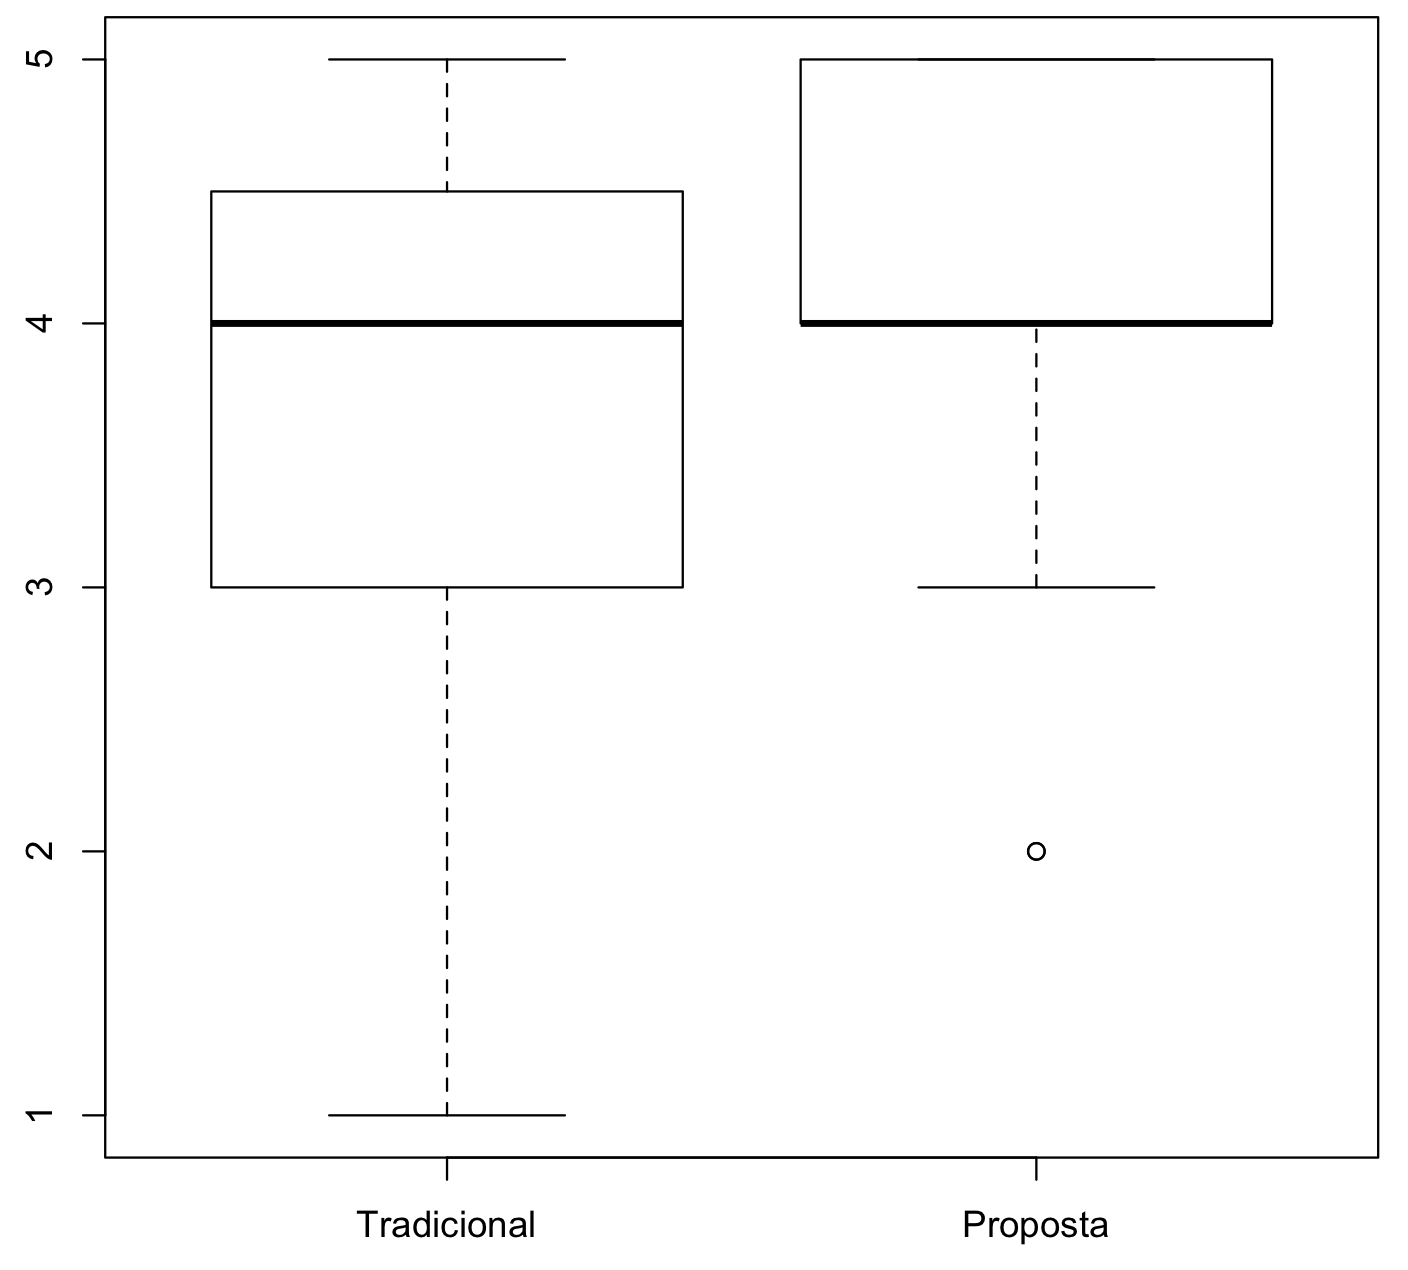
\includegraphics[scale=0.6]{./Figuras/questao3-boxplot.png}
  \end{center}
  \legend{Fonte: O autor.}
\end{figure}

Wilcoxon rank sum test with continuity correction

data:  $data\_63\_tradicional$ and $data\_63\_proposta$\\
W = 364, p-value = 0.5119\\
alternative hypothesis: true location shift is not equal to 0

\newpage
\textbf{Questão 4: As recomendações são feitas no momento adequado.}

\begin{figure}[htb]
  \caption{\label{fig:questao4-boxplot}Boxplot da questão 4}
  \begin{center}
      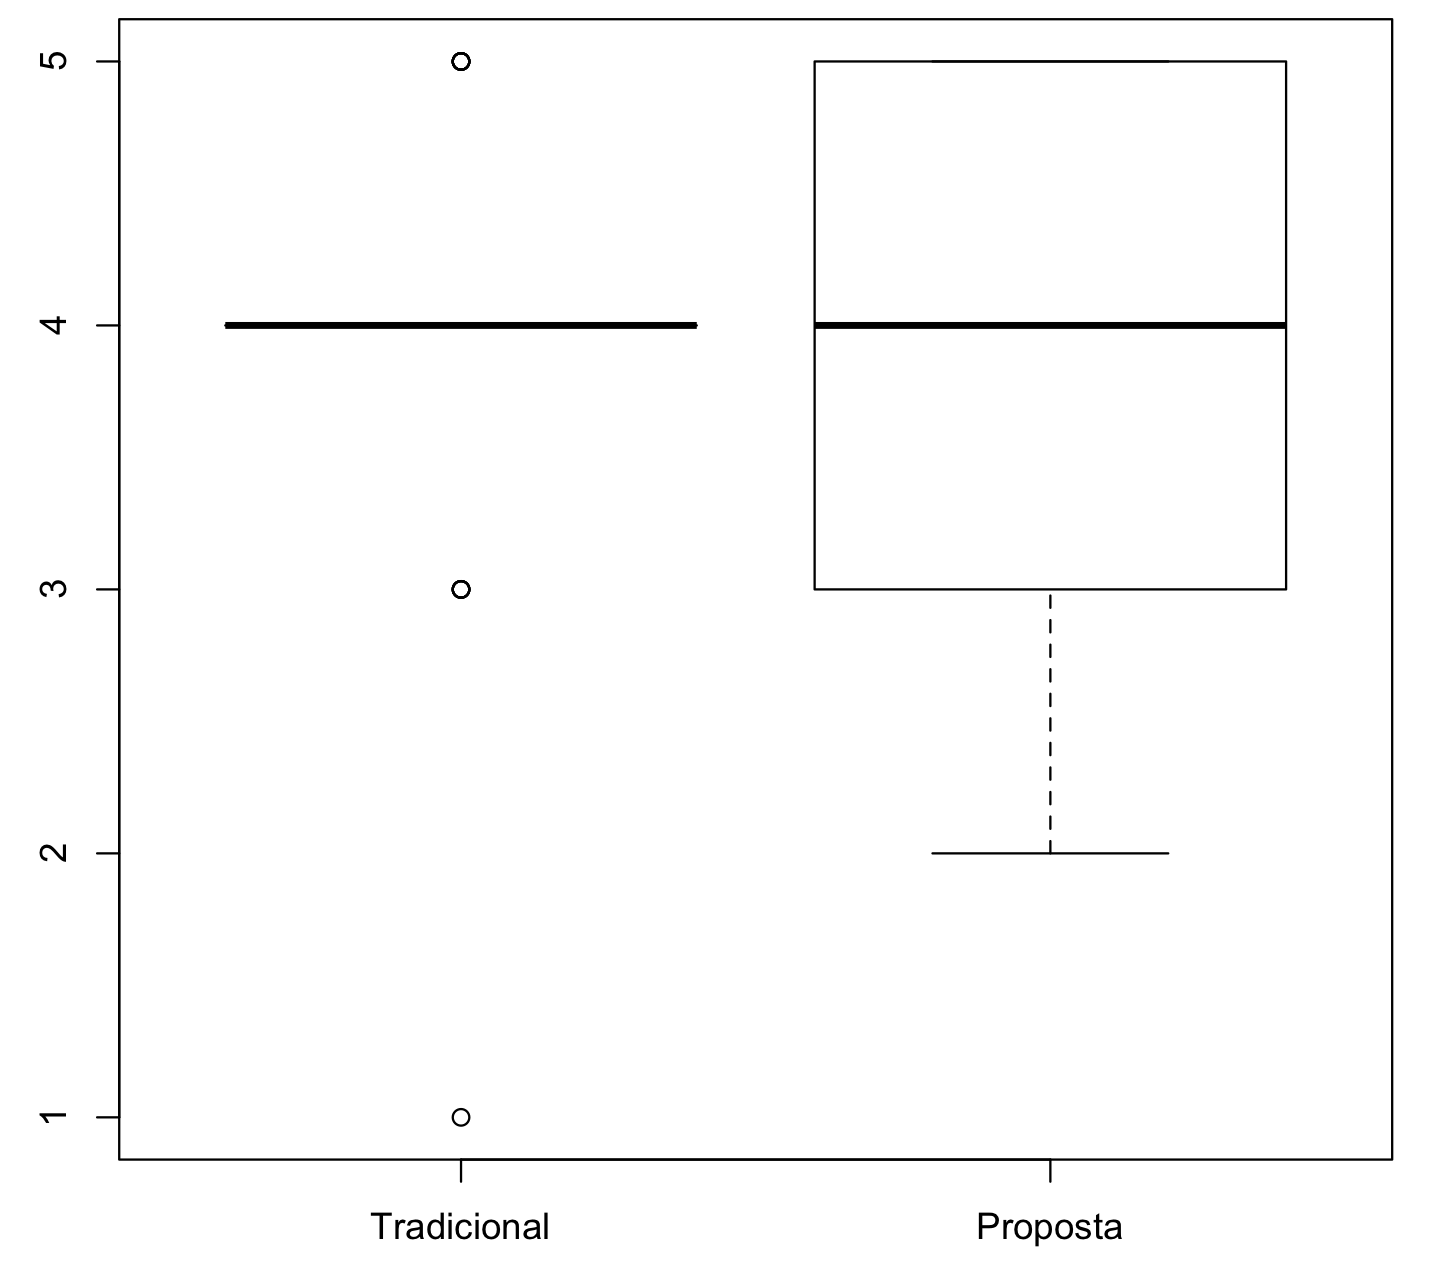
\includegraphics[scale=0.6]{./Figuras/questao4-boxplot.png}
  \end{center}
  \legend{Fonte: O autor.}
\end{figure}

Wilcoxon rank sum test with continuity correction

data:  $data\_64\_tradicional$ and $data\_64\_proposta$\\
W = 378, p-value = 0.8198\\
alternative hypothesis: true location shift is not equal to 0

\newpage
\textbf{Questão 5: O sistema de recomendação explica porque os links são recomendados para mim.}

\begin{figure}[htb]
  \caption{\label{fig:questao5-boxplot}Boxplot da questão 5}
  \begin{center}
      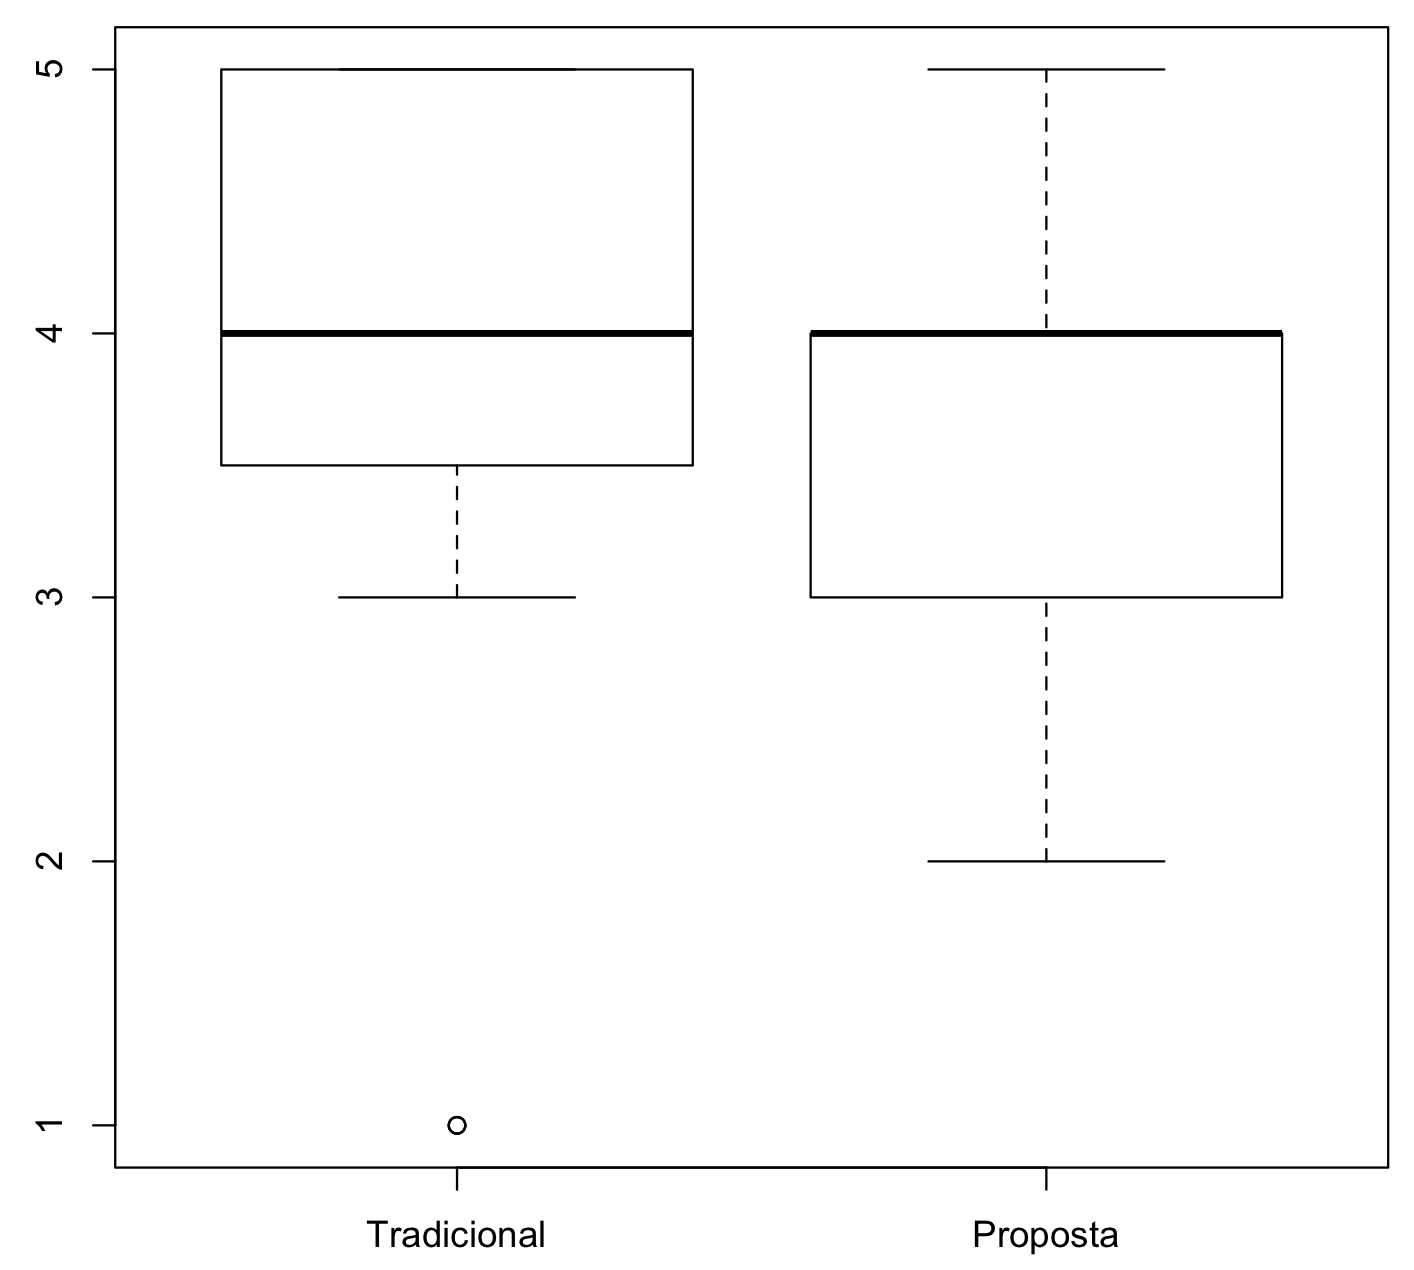
\includegraphics[scale=0.6]{./Figuras/questao5-boxplot.png}
  \end{center}
  \legend{Fonte: O autor.}
\end{figure}

Wilcoxon rank sum test with continuity correction

data:  $data\_65\_tradicional$ and $data\_65\_proposta$\\
W = 396, p-value = 0.2665\\
alternative hypothesis: true location shift is not equal to 0

\newpage
\textbf{Questão 6: A informação apresentada na interface para os itens recomendados é suficiente para mim.}

\begin{figure}[htb]
  \caption{\label{fig:questao6-boxplot}Boxplot da questão 6}
  \begin{center}
      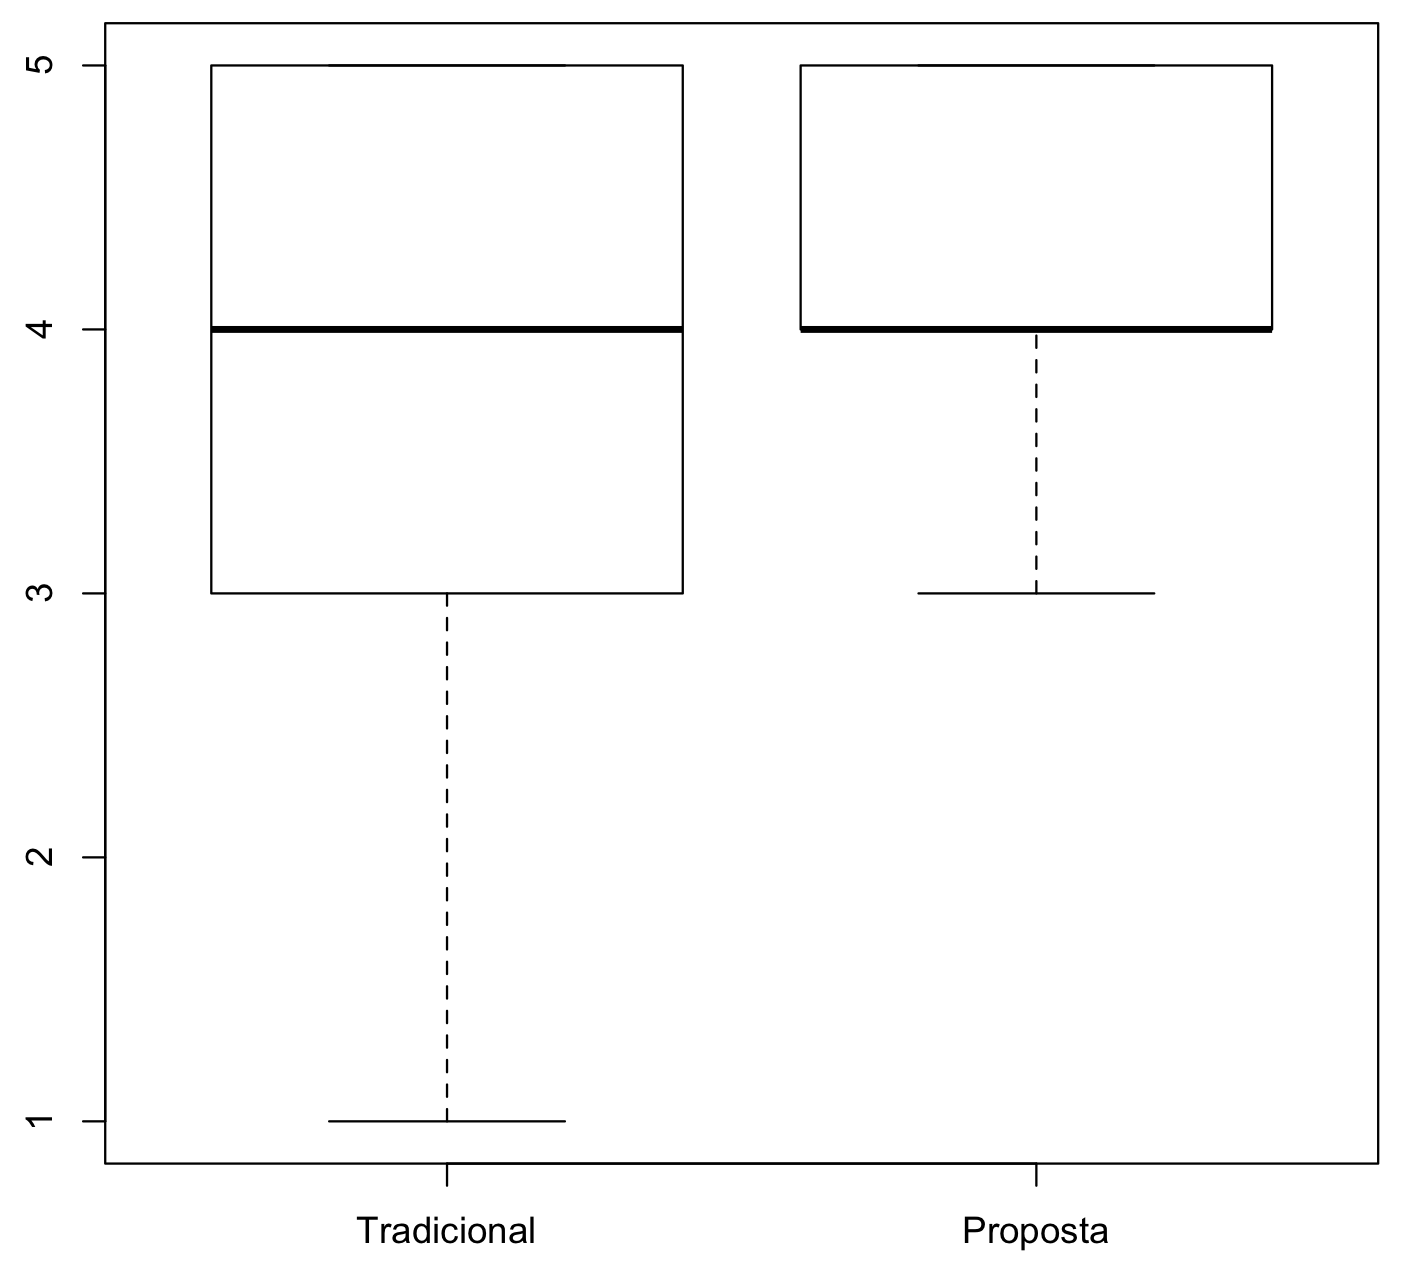
\includegraphics[scale=0.6]{./Figuras/questao6-boxplot.png}
  \end{center}
  \legend{Fonte: O autor.}
\end{figure}

Wilcoxon rank sum test with continuity correction

data:  $data\_66\_tradicional$ and $data\_66\_proposta$\\
W = 301.5, p-value = 0.1799\\
alternative hypothesis: true location shift is not equal to 0

\newpage
\textbf{Questão 7: O layout do sistema de recomendação é atrativo e adequado.}

\begin{figure}[htb]
  \caption{\label{fig:questao7-boxplot}Boxplot da questão 7}
  \begin{center}
      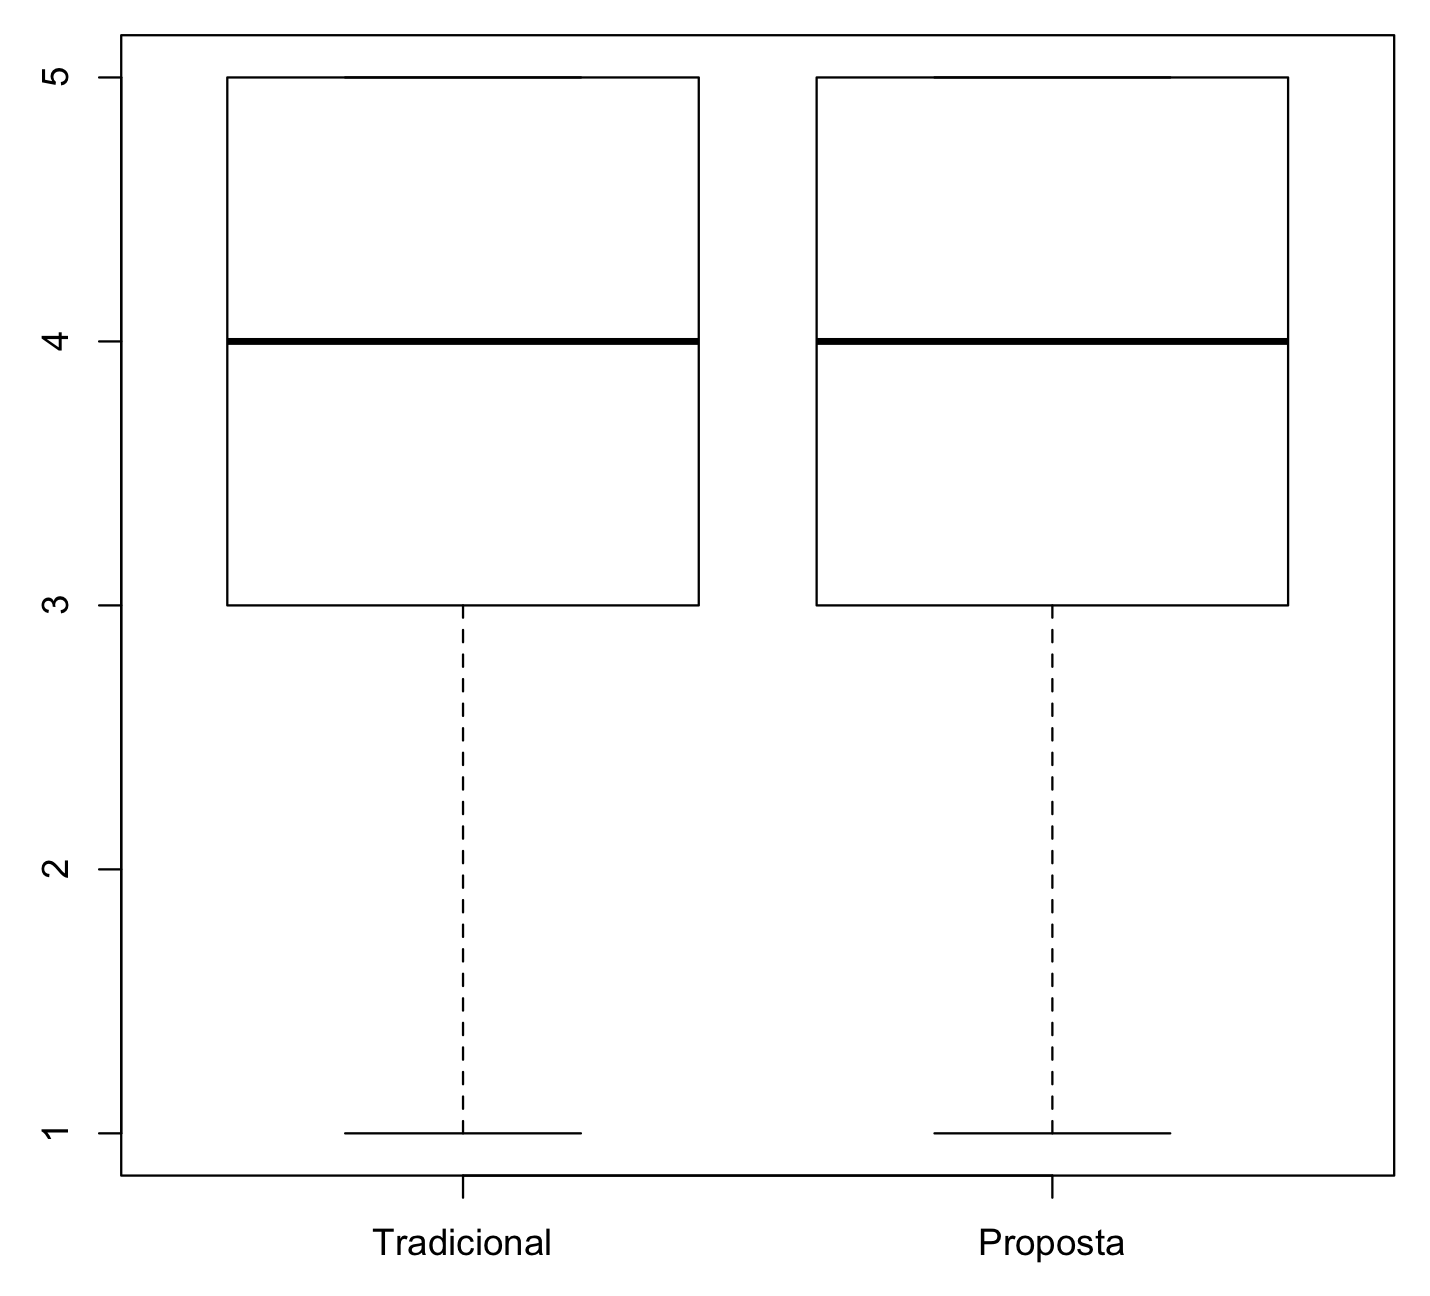
\includegraphics[scale=0.6]{./Figuras/questao7-boxplot.png}
  \end{center}
  \legend{Fonte: O autor.}
\end{figure}

Wilcoxon rank sum test with continuity correction

data:  $data\_67\_tradicional$ and $data\_67\_proposta$\\
W = 413, p-value = 0.8536\\
alternative hypothesis: true location shift is not equal to 0

\newpage
\textbf{Questão 8: Eu encontrei facilmente o local onde os itens são recomendados.}

\begin{figure}[htb]
  \caption{\label{fig:questao8-boxplot}Boxplot da questão 8}
  \begin{center}
      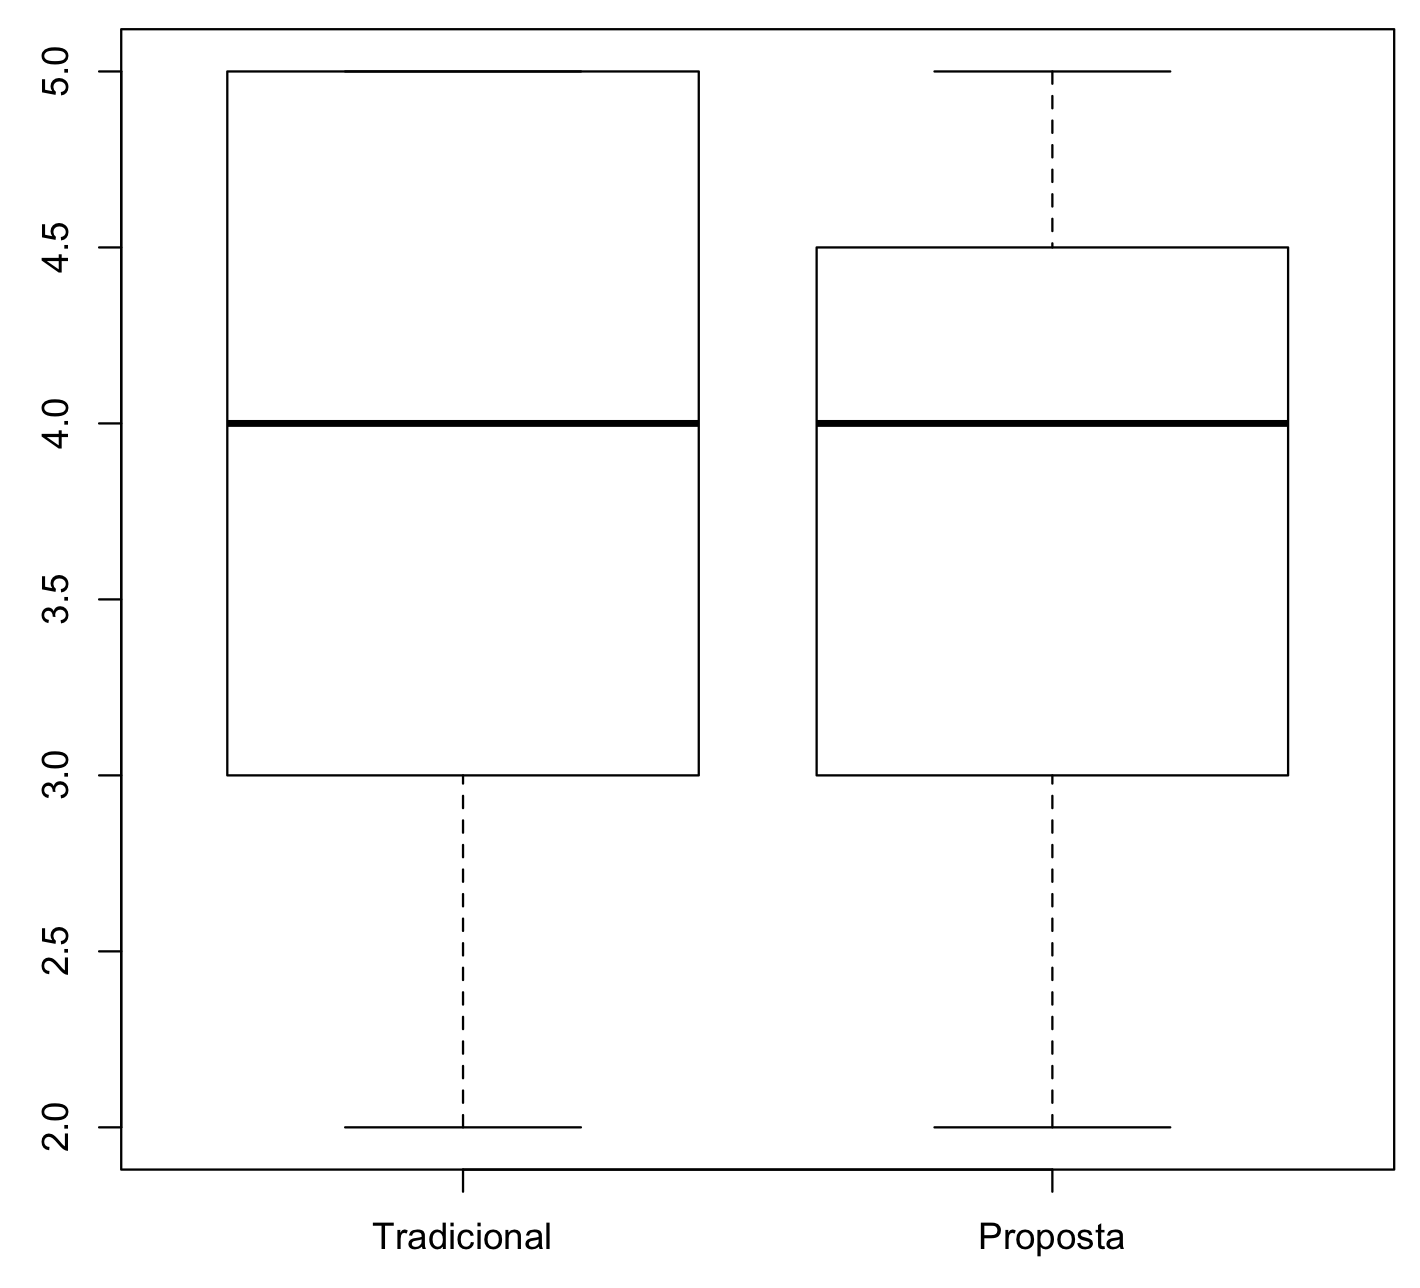
\includegraphics[scale=0.6]{./Figuras/questao8-boxplot.png}
  \end{center}
  \legend{Fonte: O autor.}
\end{figure}

Wilcoxon rank sum test with continuity correction

data:  $data\_68\_tradicional$ and $data\_68\_proposta$\\
W = 381, p-value = 0.7093\\
alternative hypothesis: true location shift is not equal to 0

\newpage
\textbf{Questão 9: Eu percebi que o sistema de recomendação aprendia sobre minhas necessidades/preferências conforme eu avançava na disciplina.}

\begin{figure}[htb]
  \caption{\label{fig:questao9-boxplot}Boxplot da questão 9}
  \begin{center}
      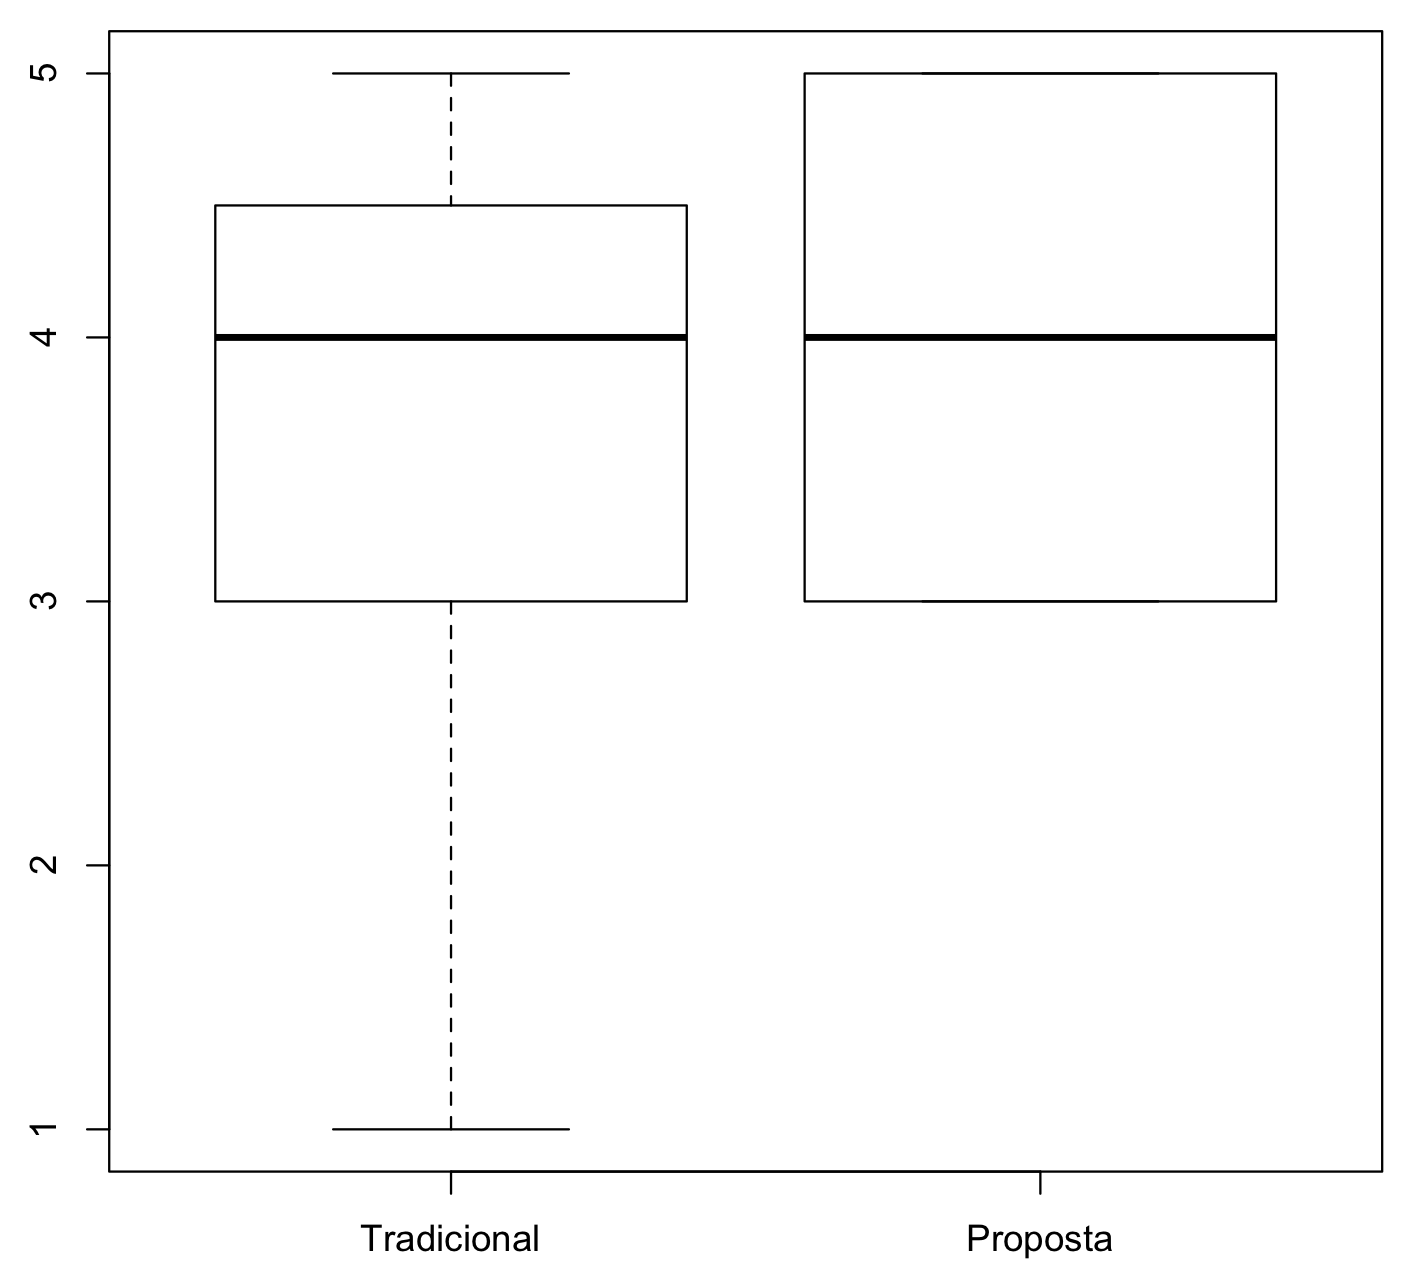
\includegraphics[scale=0.6]{./Figuras/questao9-boxplot.png}
  \end{center}
  \legend{Fonte: O autor.}
\end{figure}

Wilcoxon rank sum test with continuity correction

data:  $data\_69\_tradicional$ and $data\_69\_proposta$\\
W = 313.5, p-value = 0.6722\\
alternative hypothesis: true location shift is not equal to 0

\newpage
\textbf{Questão 10: É facil encontrar um item para estudar com a ajuda do sistema de recomendação.}

\begin{figure}[htb]
  \caption{\label{fig:questao10-boxplot}Boxplot da questão 10}
  \begin{center}
      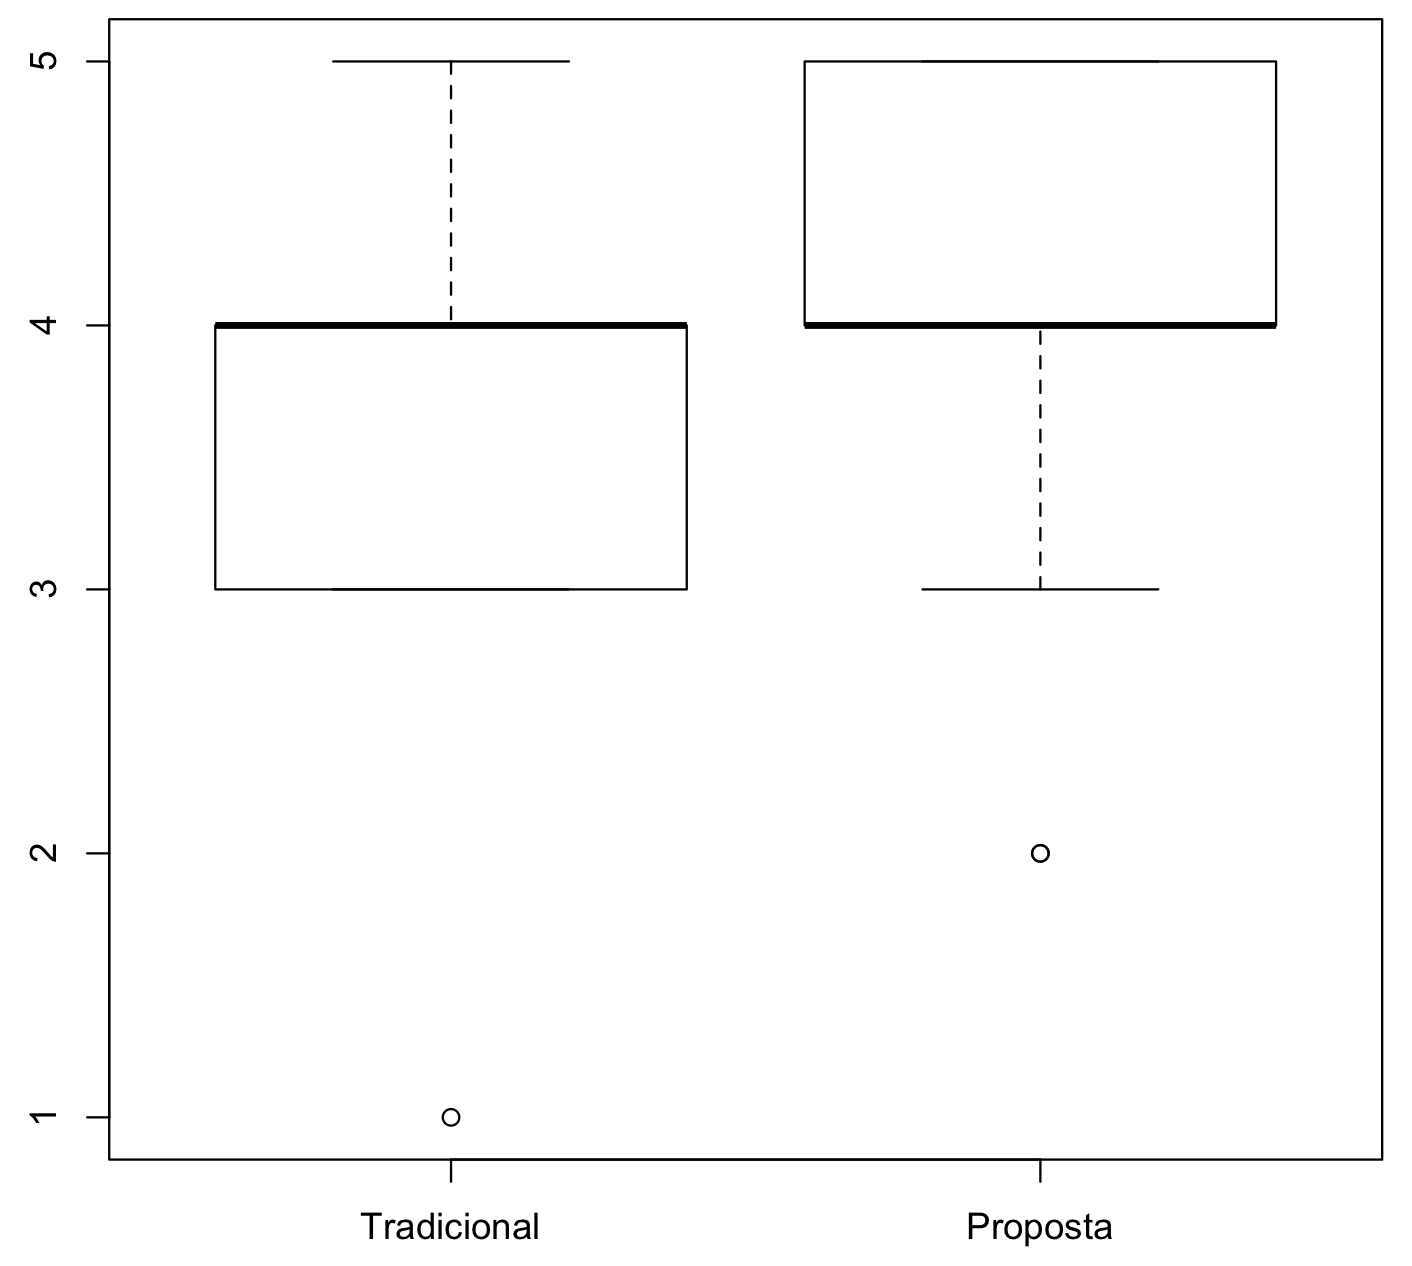
\includegraphics[scale=0.6]{./Figuras/questao10-boxplot.png}
  \end{center}
  \legend{Fonte: O autor.}
\end{figure}

Wilcoxon rank sum test with continuity correction

data:  $data\_70\_tradicional$ and $data\_70\_proposta$\\
W = 296, p-value = 0.1452\\
alternative hypothesis: true location shift is not equal to 0

\newpage
\textbf{Questão 11: Eu me senti apoiado para encontrar itens do meu interesse com a ajuda do sistema de recomendação.}

\begin{figure}[htb]
  \caption{\label{fig:questao11-boxplot}Boxplot da questão 11}
  \begin{center}
      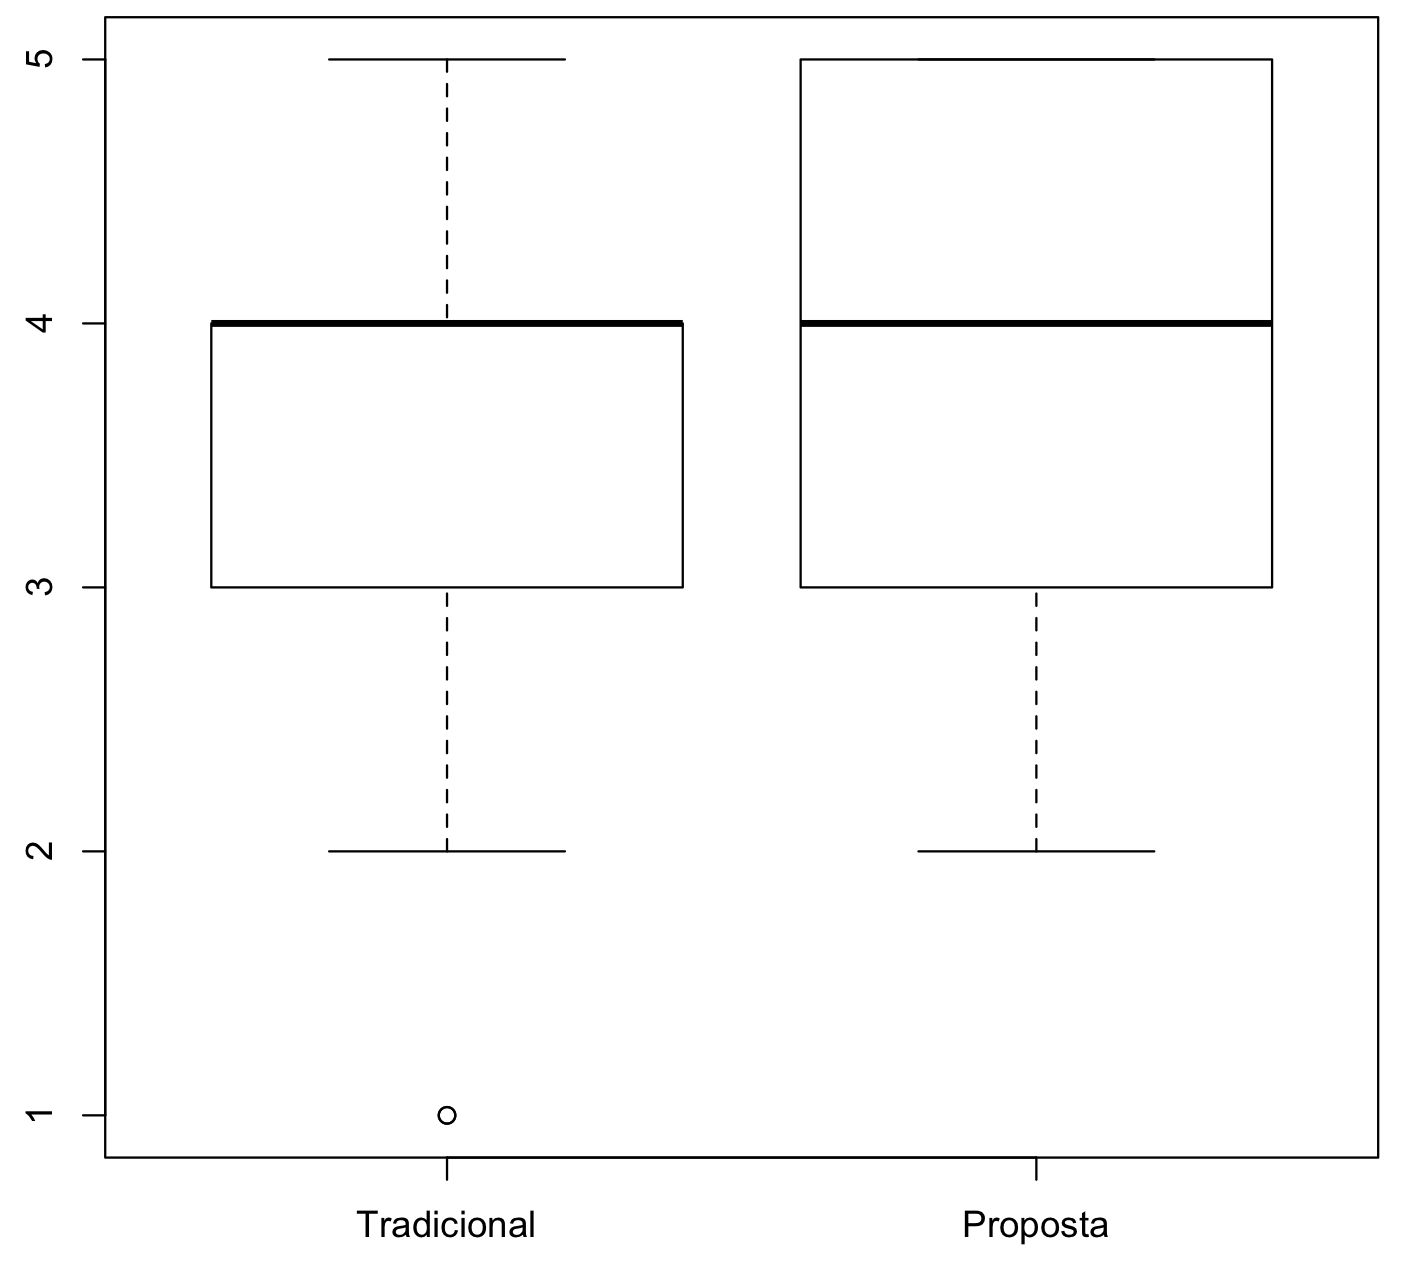
\includegraphics[scale=0.6]{./Figuras/questao11-boxplot.png}
  \end{center}
  \legend{Fonte: O autor.}
\end{figure}

Wilcoxon rank sum test with continuity correction

data:  $data\_71\_tradicional$ and $data\_71\_proposta$\\
W = 286, p-value = 0.2309\\
alternative hypothesis: true location shift is not equal to 0

\newpage
\textbf{Questão 12: Eu entendi porque os itens foram recomendados para mim.}

\begin{figure}[htb]
  \caption{\label{fig:questao12-boxplot}Boxplot da questão 12}
  \begin{center}
      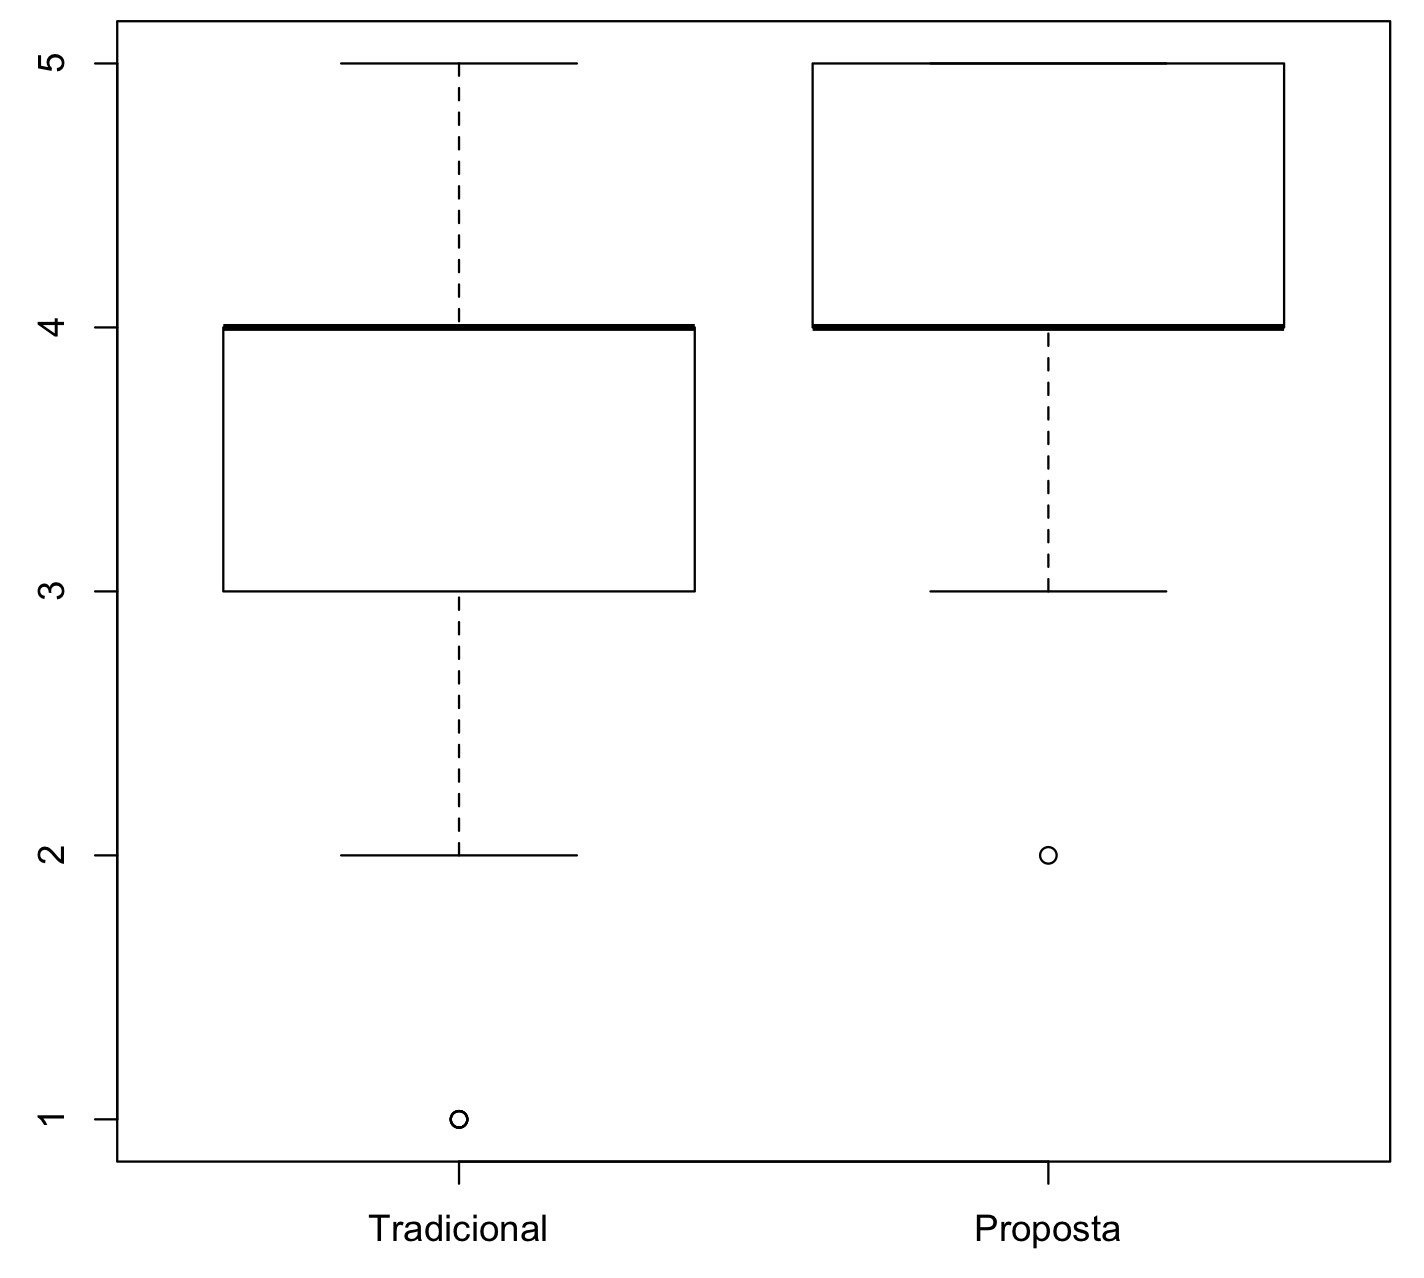
\includegraphics[scale=0.6]{./Figuras/questao12-boxplot.png}
  \end{center}
  \legend{Fonte: O autor.}
\end{figure}

Wilcoxon rank sum test with continuity correction

data:  $data\_72\_tradicional$ and $data\_72\_proposta$\\
W = 240, p-value = 0.01513\\
alternative hypothesis: true location shift is not equal to 0

\newpage
\textbf{Questão 13: No geral, estou satisfeito com o sistema de recomendação.}

\begin{figure}[htb]
  \caption{\label{fig:questao13-boxplot}Boxplot da questão 13}
  \begin{center}
      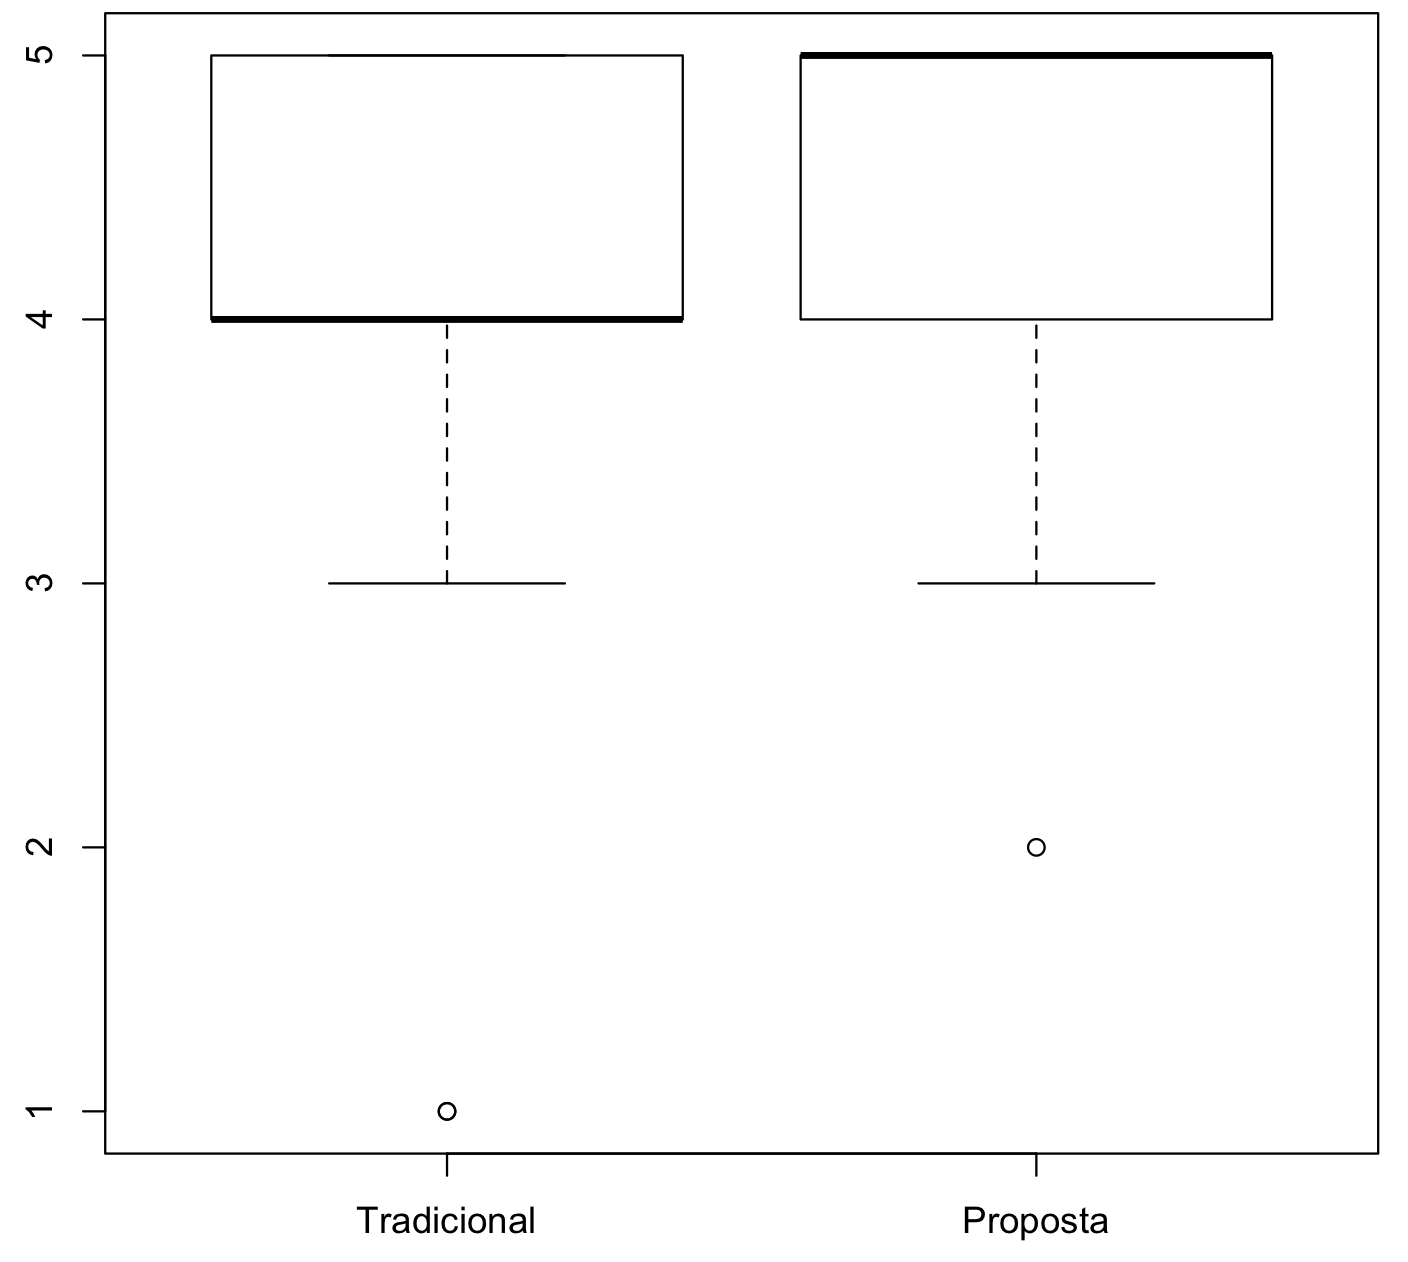
\includegraphics[scale=0.6]{./Figuras/questao13-boxplot.png}
  \end{center}
  \legend{Fonte: O autor.}
\end{figure}

Wilcoxon rank sum test with continuity correction

data:  $data\_73\_tradicional$ and $data\_73\_proposta$\\
W = 356.5, p-value = 0.2388\\
alternative hypothesis: true location shift is not equal to 0
